\chapter{Adăugare funcție de grosime și analiza în tandem}\label{chapter:grosime}

\section{Adăugare funcție de grosime}

Metodologia de proiectare a paletelor subțiri oferă axa curbată a paletei. În cazul profilelor reale, grosimea trebuie adăugată la această formă pentru a asigura integritatea structurală. Pentru lucrarea de față am adoptat distribuția grosimii YS-900 a hidro profilelor \cite{eppler1979wing} pentru grosimea paletei în direcția tangențială. Funcția de grosime este dimensionată pentru un blocaj maxim de 10\% la o lățime axială de 52,5\% de la frontul rețelei. Statorul gros și paletele rotorului sunt reprezentate în figura 5.1.. O optimizare directă a paletelor groase folosind abordarea similară utilizată în această lucrare a fost încercată și în \cite{frunzua2010optimization}.

Subliniem faptul că grosimea paletei, considerată în mod tradițional în direcția normală locală față de linia de coardă, este obținută prin aplicarea grosimii tangențiale alese, împrumutate de la un profil simetric.

\begin{figure}[h]
  \centering
  \begin{subfigure}[t]{0.4\textwidth}
    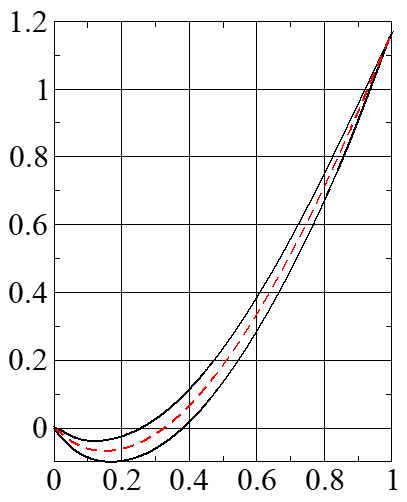
\includegraphics[width=\textwidth]{figures/stator-thick-blade.PNG}
  \end{subfigure}
  \begin{subfigure}[t]{0.42\textwidth}
    \hspace{2pt}
    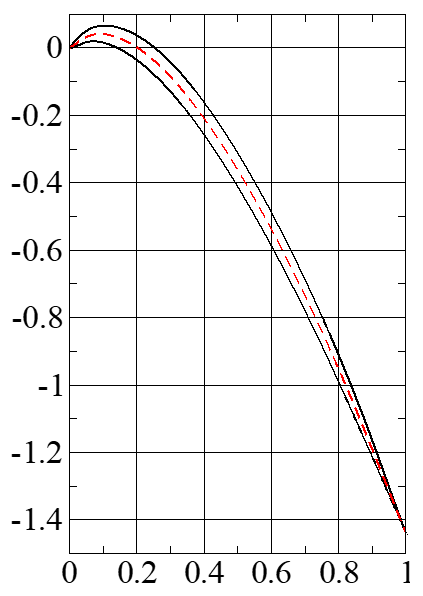
\includegraphics[width=\textwidth]{figures/rotor-thick-blade.PNG}
  \end{subfigure}
  \caption{Profile cu funcție de grosime pentru stator (stânga) și rotor (dreapta)}
\end{figure}

\begin{figure}
	\centering
	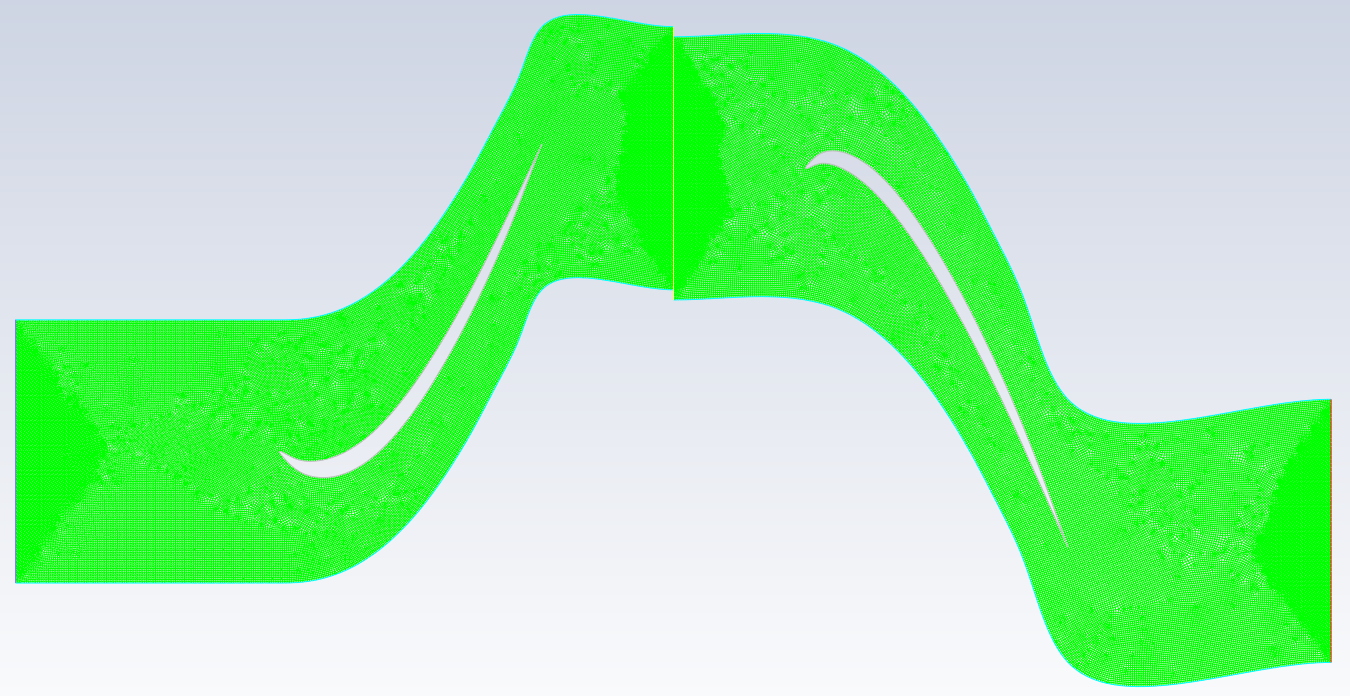
\includegraphics[scale=0.4]{figures/tandem_thick_mesh.PNG}
	\caption{Discretizare în tandemul stator rotor cu funcție de grosime}
	\label{Discretizare în tandemul stator rotor cu funcție de grosime}
\end{figure}


Tandemul rotor-stator cu profile groase este evaluat în o simulare cu fluid vâscos discretizarea căruia se poate observa în Figura 5.2., folosind în cazul nostru modelul de turbulență Spalart și Allmaras \cite{spalart1992one} conform figurii 5.3.

\begin{figure}
	\centering
	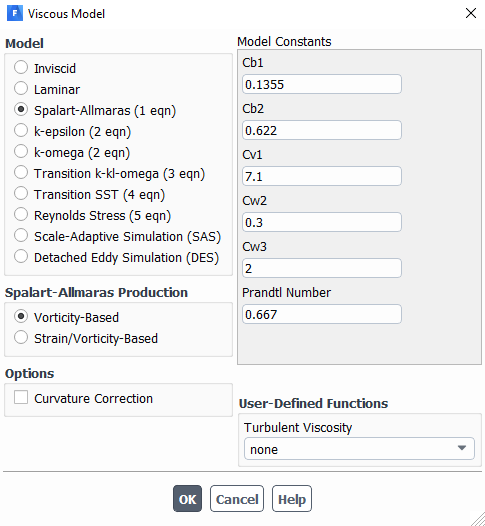
\includegraphics[scale=0.7]{figures/tandem_thick_viscous_model.PNG}
	\caption{Modelul de vâscozitate ales}
	\label{Modelul de vâscozitate ales}
\end{figure}

Figura 5.4. reprezintă harta de distribuție a presiunii totale obținută în acest caz, ca o ilustrare a evoluției specifice a energiei hidraulice în regiunea cu palete. În amonte de paletele rotorului, presiunea totală rămâne practic constantă, cu excepția straturilor de graniță. În zona paletelor rotorului, presiunea totală scade, corespunzând conversiei energiei hidraulice în energia mecanică. De asemenea, presiunea totală are o creștere la bordul de atac (pete roșii) care sunt o prezentă obișnuită în turbinele de acest fel.

\begin{figure}
	\centering
	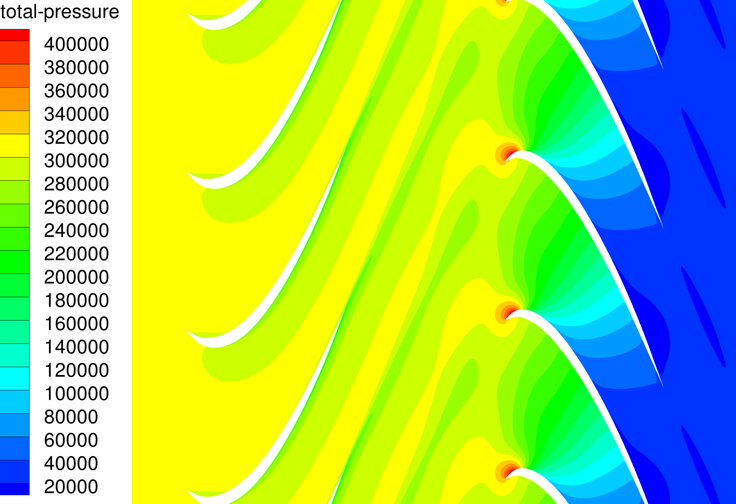
\includegraphics[scale=1]{figures/presiunea-totala.png}
	\caption{Presiunea totală în tandemul stator rotor}
	\label{Presiunea totală în tandemul stator rotor}
\end{figure}